
%307
\chapter{Модули над кольцами\\главных идеалов}
\noindent В этой и следующих главах факторгруппа $\mathbb{Z}/n\mathbb{Z}$ будет давольно ча-\linebreak
сто появляться по очевидным причинам для представления$(\mathbb{Z}/180\mathbb{Z}\simeq$ \linebreak
 $\mathbb{Z}/2^2\mathbb{Z}\times \mathbb{Z}/3^2\mathbb{Z}\times \mathbb{Z}/5\mathbb{Z})$. Необходимо упрощение описания: обозначение \linebreak
  $\mathbb{Z}_n$ --- не всегда, в действительности, традиционное --- отведено при \linebreak простом $n$ для кольца частных из $\mathbb{Z}$ со знаменателем из $\mathbb{Z}-n\mathbb{Z}$. При \linebreak необходимости, во избежании путаницы, оно будет дополнительно ого- \linebreak ворено.  

Для студента --- математика теория модулей над кольцами главных \linebreak идеалов (с классификацией через инвариантные множетели) часто вос- \linebreak принимается как трудная: формулировки результатов кажутся заум-\linebreak ными, а доказательства слишком техничными. В этом введении абелева \linebreak группа $\mathbb{Z}_n \times \mathbb{Z}_m$ является простой изучаемой моделью, которая позволит \linebreak нам попытаться разобраться в этой теории. Основным инструментом в \linebreak теории модулей является соотношение Безу: можно сказать, что любая \linebreak теория $\ll$основывается$\gg$ на умении пользоваться этим соотношением. Но \linebreak начнем с начала. Любой студент математического факультета второго \linebreak курса университета слышал о китайской теореме: 
\begin{thm}[китайская теорема об остатках (нулевая или минимальная\linebreak форма)]

Если $n$ и $m$ - два \textit{ взаимно простых целых числа}, то абелевы группы \linebreak $\mathbb{Z}_n \times\mathbb{Z}_m\times\mathbb{Z}_{nm}$ изоморфны.
\end{thm}
  Читатель, интересующийся историей китайской теоремы, может \linebreak обратиться к работе Диксона $\ll$ History of the theory of numbers $\gg$ или к работе Марцлоффа $\ll$ Histoire des mathématiques chinoises $\gg$ ; из последней \linebreak можно узнать, что в $\ll$ Суан-Шинь $\gg$ китайский классик арифметики Сунь \linebreak Цу, живший в первом веке нашей эры, формулирует в форме туманной 
%308
поэмы: \textit{$\ll$...gave in the form of an obscure verse a rule called t'ai-yen (great\linebreak generalisation) to determine a number hfving the remainders...$\gg$\footnote{$\ll$...дано в виде туманного стиха правило, называемое тай-йен (великое обощение), нахождения числа, имеющего остатки...$\gg$}} правило \linebreak определения числа, имеющего остатками 2, 3, 3, соответственно, при де- \linebreak лении на 3, 5, 7, что приводит к числу 23. Связь между этой проблемой \linebreak и абстрактной формулировкой китайской теоремы объясняется далее.\linebreak Рибейнбойм в книге $\ll$The Book of Prime Number Records$\gg$ указывает так- \linebreak же, что эта теорема позволяла китайским генералам пересчитать свою \linebreak армию без особых усилий, распоряжаясь: $\ll$выстраивайтесь в ряд 7 за\linebreak 7 (по 7), затем 11 за 11, затем 12 за 13 и, наконец, 17 за 17$\gg$. Если эта \linebreak история верна, то можно вывести максимальное число солдат в армии \linebreak и даже насколько велико было оживление во время пеерсчера, но это \linebreak уже другая история. Китайская теорема может быть сформулирована \linebreak в другом, более точном, виде, где появляется изоморфизм:  
\begin{thm}[Китайская теорема об остатках (форма 1)]

  Если $n$ и $m$ - два взаимно простых целых числа, то отображение\linebreak
$\mathbb{Z}_{nm}\ni \overline{x_{nm}}\mapsto(\overline{x_n},\overline{x_m}\in \mathbb{Z}_n \times\mathbb{Z}_m$, где $\overline{x_n}$ обозначает класс $x \in \mathbb{Z}$ по \linebreak модулю $n$, является корректно определенным изоморфизмом групп. В \linebreak действительности, это изоморфизм \textbf{колец}.
 \end{thm}
  Можно дать китайской теореме простую формулировку, в которой \linebreak нет ни групп, ни изоморфизмов:   
\begin{thm}[Китайская теорема об остатках (форма 2)]

  Пусть $n$ и $m$ - два взаимно простых целых числа; для данных целых \linebreak чисел $y$, $z$ система

\begin{equation*}
S(y, z) : 
\begin{cases}
    x \equiv y\pmod{n}, \\
    x \equiv z\pmod{m} \\
\end{cases}
\end{equation*}

имеет решение $x \in \mathbb{Z}$; кроме того, $x'\in \mathbb{Z}$ будет другим решением тогда \linebreak и только тогда, когда $x \equiv x'\pmod{nm}$.
\end{thm}
  Эта последняя формулировка,более точная, чем предыдущая, со- \linebreak держит следующую структурную информацию: решение $x$ по модулю \linebreak $nm$ аддитивно и мультипликативно зависит от двух данных значений $y$ и $z$.
  Благодаря этой формулировке приходим к загадке: $\ll$я выбрал чи-\linebreak сло не более, чем из двух цифр; при делении этого числа на 9 и на\linebreak 11 получил соответственно остатки 4 и 8; можете ли вы мне ска- \linebreak зать какое это число?$\gg$, математик может ответить в стиле, достой-\linebreak Пьера Дака и Франциса Бланша: \textit{$\ll$ да, я могу его назвать; более
%309
того, могу сказать, что такое число, имеющее самое большее две \linebreak цифры, единственно!$\gg$}. Благодаря этой тираде, читатель уже понял,\linebreak что формулировка китайской теоремы, приведенные выше, недоста-\linebreak точны для эффективного решения системы $S(y,z)$. Это решение, свя-\linebreak занное с умением выразить в явном виде обратимость изоморфизма\linebreak $\mathbb{Z}_{nm}\ni \overline{x_{nm}}\mapsto(\overline{x_n},\overline{x_m}\in \mathbb{Z}_n \times\mathbb{Z}_m$, задает, впрочем, соотношение Безу, \linebreak которое нам известно из главы 2. Действительно, начиная с соотноше-\linebreak ния Безу для $n$ и $m$: $1=un+vm$, легко выделить системы:
$$ \left\{
\begin{array}{rcl}
vm \equiv 1&(\bmod{n}),\\
vm \equiv 0&(\bmod{m})\\
\end{array}
\right. и 
\left\{
\begin{array}{rcl}
un \equiv 0&(\bmod{n}),\\
un \equiv 1&(\bmod{m}).\\
\end{array}
\right.$$
В других терминах,$vm$ - решение системы $S(1,0)$ и $un$ - решение \linebreak системы $S(0,1)$; в силу линейности, в чем читатель может убедиться \linebreak сам, $x=yvm+zun$ - решение системы $S(y,z)$.
  
  Таким образом, для $n=9$, $m=11$ имеет место соотношение Безу \linebreak $1=5\times 9+(-4)\times 11$, которое представляет число $x=4\times (-44)+ \linebreak +8 \times 45=184$ как решение системы $S(4,8)$;это решение может быть \linebreak приведено по модулю $9 \times 11 = 99$; и получим число 85 как ответ на \linebreak загадку, приведенную выше.
  
  Китайская теорема является частным случаем применения теории \linebreak инвариантных множителей: если $n$ и $m$ взаимно просты, число $nm$ пол-\linebreak ностью определяет структуру группы $\mathbb{Z}_n \times \mathbb{Z}_m$. Таким образом, если $n'$ \linebreak и $m'$ также взаимно просты, то:
$$\mathbb{Z}_n \times \mathbb{Z}_m \simeq \mathbb{Z}_{n'} \times \mathbb{Z}_{m'} \Longleftrightarrow nm=n'm'.$$
  
  Нас сейчас интересует структура абелевой группы $\mathbb{Z}_n \times \mathbb{Z}_m$ для про- \linebreak извольных $n$ и $m$ (не обязательно взаимно простых и, возможно, ну-\linebreak левых). Как, например, эффективно решить вопрос о существовании \linebreak изоморфизма между $\mathbb{Z}_n \times \mathbb{Z}_m$ и  $\mathbb{Z}_{n'} \times \mathbb{Z}_{m'} \Longleftrightarrow nm=n'm'$? Первая часть ответа на этот \linebreak вопрос заключается в следующей теореме, следствии из китайской те-\linebreak оремы, т.е. в следствии из соотношения Безу.
\begin{thm}[Структурная теорема (нормализованная форма произведения двух циклических групп)]

  Если $n$ и $m$ - два целых числа, то существует изоморфизм групп\linebreak $\mathbb{Z}_n \times \mathbb{Z}_m$ и $\mathbb{Z}_{n \wedge m} \times \mathbb{Z}_{n \vee m}$; запись  $n \wedge m$ обозначает наибольший общий \linebreak делитель $m$ и $n$; $n \vee m$ - наименьшее общее кратное. Если $n$ и $m$ взаимно \linebreak просты, то абелевы группы $\mathbb{Z}_n \times \mathbb{Z}_m$ и $\mathbb{Z}_{nm}$ изоморфны.
\end{thm}
\newpage
%310
\begin{myproof}
Разложим $n$ (соответственно $m$) в произведение простых чисел \linebreak(используя нулевые показатели, чтобы в записи фигурировали все \linebreak необходимые начальные простые числа):
$$n={p_1}^{\alpha_1}{p_2}^{\alpha_2}...{p_k}^{\alpha_k} (\alpha_i \ge 0), m={p_1}^{\beta
_1}{p_2}^{\beta_2}...{p_k}^{\beta_k} (\beta_i \ge 0)$$
($p_i$ простые числа).
Тогда имеют место изоморфизмы:
$$\mathbb{Z}_n \simeq \mathbb{Z}_{{p_1}^\alpha_1} \times \mathbb{Z}_{{p_2}^\alpha_2} \times ... \times \mathbb{Z}_{{p_k}^\alpha_k}, \mathbb{Z}_m \simeq \mathbb{Z}_{{p_1}^\beta_1} \times \mathbb{Z}_{{p_2}^\beta_2} \times ... \times \mathbb{Z}_{{p_k}^\beta_k}$$
и, как следствие, группа $\mathbb{Z}_n \times \mathbb{Z}_m$ изоморфна
$$\mathbb{Z}_{{p_1}^{\inf(\alpha_1, \beta_1)}} \times \mathbb{Z}_{{p_2}^{\inf(\alpha_2, \beta_2)}} \times ... \times \mathbb{Z}_{{p_k}^{\inf(\alpha_k, \beta_k)}}\linebreak \times \mathbb{Z}_{{p_1}^{\sup(\alpha_1, \beta_1)}} \times \mathbb{Z}_{{p_2}^{\sup(\alpha_2, \beta_2)}} \times ... \times \mathbb{Z}_{{p_k}^{\sup(\alpha_k, \beta_k)}},$$
т.е. она изоморфна группе $\mathbb{Z}_{n \wedge m} \times \mathbb{Z}_{n \vee m}$.
\end{myproof}
  В разделе 2.3 мы докажем, что среди всех групп $\mathbb{Z}_{n'} \times \mathbb{Z}_{m'}$, изо- \linebreak морфных данной группе $\mathbb{Z}_{n} \times \mathbb{Z}_{m}$, существует единственная группа, для \linebreak которой $n'$ делит $m'$, и эта группа $\mathbb{Z}_{n \wedge m} \times \mathbb{Z}_{n \vee m}$. Покажем, как этот ре-\linebreak зультат может служить для определения группы  $\mathbb{Z}_{n} \times \mathbb{Z}_{m}$; рассмотрим,\linebreak например, $n=180=2^2 \cdot 3^2 \cdot 5$ и $m=600=2^3 \cdot 3 \cdot 5^2$:
$$\mathbb{Z}_{180} \simeq \mathbb{Z}_{2^2} \times \mathbb{Z}_{3^2} \times \mathbb{Z}_{5}, \mathbb{Z}_{600} \simeq \mathbb{Z}_{2^3} \times \mathbb{Z}_{3} \times \mathbb{Z}_{5^2},$$
и, следовательно, $\mathbb{Z}_{180} \times \mathbb{Z}_{600}$ изоморфна $\mathbb{Z}_{2^2 \times 3 \times 5} \times \mathbb{Z}_{2^3 \times 3^2 \times 5^2}$, т.е. груп-\linebreak пе $\mathbb{Z}_{60}\times \mathbb{Z}_{1800}$. Если мы проделаем аналогичную операцию для чисел \linebreak $n = 360$ и $m = 300$, то мы найдем $\mathbb{Z}_{360} \times \mathbb{Z}_{300} \simeq \mathbb{Z}_{60} \times \mathbb{Z}_{1800}$. Абелевы \linebreak группы $\mathbb{Z}_{180} \times \mathbb{Z}_{600}$ и $\mathbb{Z}_{360}\times \mathbb{Z}_{300}$ имеют порядок $108000$, и, следователь-\linebreak но, они изоморфны, так как они обе изоморфны группе $\mathbb{Z}_{60} \times \mathbb{Z}_{1800}$.
  
  И напоследок, применяя ту же операцию к группе $\mathbb{Z}_{240} \times \mathbb{Z}_{450}$, име-\linebreak ющей тот же порядок $108000$, получаем $\mathbb{Z}_{240} \times \mathbb{Z}_{450} \simeq \mathbb{Z}_{30} \times \mathbb{Z}_{3600}$ c \linebreak $30 \mid 3600$, и в силу единственности, последняя группа $\mathbb{Z}_{240} \times \mathbb{Z}_{450}$ не \linebreak будет изоморфна предыдущим.
  
  Внимательный читатель может заметить, что в структурной тео-\linebreak реме, приведенной выше, явный вид изоморфизма между $\mathbb{Z}_{n}\times \mathbb{Z}_{m}$ и \linebreak $\mathbb{Z}_{n \wedge m} \times \mathbb{Z}_{n \vee m}$ не виден. Чтобы успокоить читателя, отметим, что он \linebreak появится позже. \newpage
%311
\section{Исключение и несколько следствий.}
В этом разделе мы покажем как рабочие $\ll$инструменты$\gg$ для изучения \linebreak приведения к каноническому виду матриц с целыми элементами, так \linebreak и первые приложения, одни из которых имеют абстрактный характер\linebreak (модуль без кручения конечного типа), а другие --- конкретный (вычи-\linebreak сление определителей). 
  
  Напомним, что квадратная матрица обратима тогда и только тогда, \linebreak когда ее определитель обратим в кольце элементов. Кольцо предпо-\linebreak лагается коммуникативным и с единицей. Будем использовать следующие обозначения:
\begin{itemize}
  \item $M(n, m, A)$ и $M_{n,m}(A)$ для модуля матриц размеров $n\times m$ с
  элементами из кольца $A$,
  \item  $M(m,A)$ и $M_m(A)$ для кольца матриц размеров $m\times m$ с
  элементами  из кольца $A$,
  \item  $GL(m,A)$ и $GL_m(A)$ для групп матриц размеров $m\times m$ с 
  элементами из кольца $A$ и обратимых в $M_m(A)$,
  \item  $SL(m,A)$ и $SL_m(A)$ для подгруппы группы $GL_m(A)$, состоящей 
  из матриц с определителем $1$.
  \end{itemize}
\subsection{Операции над строками и столбцами матрицы}

Пусть даны два индекса $j$ и $k$ и четыре элемента $\alpha$, $\beta$, $\gamma$, $\delta$ из коль-\linebreak ца; обозначим через ${\left( \begin{array}{ccc}
\alpha & \beta \\
\gamma & \delta \\
\end{array} \right)}_{jk}$ квадратичную матрицу, описанную ниже. По контексту понятно, как определить размеры этой квадратной матри- \linebreak цы. Определим матрицу 
${\left( \begin{array}{ccc}
\alpha & \beta \\
\gamma & \delta \\
\end{array} \right)}_{jk}$:

\begin{tabular}{llll}
\multicolumn{3}{l}{${\left( \begin{array}{ccc}
\alpha & \beta \\
\gamma & \delta \\
\end{array} \right)}_{jk} (e_i)=e_i для l\neq j,k, 
\
$}     & \multirow{3}{*}{\bordermatrix{
& & & \underset{\downarrow}{j} & & \underset{\downarrow}{k} & & \cr
& 1 & 0 & & & & 0 & 0\cr
& 0 & \ddots & & & & & 0 \cr
j\to & & & \alpha & & \beta & & \cr
& \vdots & & & & & & \vdots \cr
k\to & & & \gamma & & \delta & & \cr
& & & & & & \ddots & 0 \cr
& 0 & 0 & & & & 0 & 1 \cr}} \\
\multicolumn{3}{l}{${\left( \begin{array}{ccc}
\alpha & \beta \\
\gamma & \delta \\
\end{array} \right)}_{jk} (e_j)=\alpha e_j + \gamma e_k,$ }    &                   \\
\multicolumn{3}{l}{${\left( \begin{array}{ccc}
\alpha & \beta \\
\gamma & \delta \\
\end{array} \right)}_{jk} (e_k)=\beta e_j + \delta e_k,$} &                  
\end{tabular}
\newpage
семейство $(e_i)_{1\le i \le n}$ обозначает, конечно, канонический базис.
  
  Напомним, что комбинирование строк (соответственно столбцов)\linebreak матрицы эквивалентно умножению этой матрицы слева (соответствен- \linebreak но справа) на некоторую матрицу.
%312
\begin{predl}  
  Определитель матрицы ${\left( \begin{array}{ccc}
\alpha & \beta \\
\gamma & \delta \\
\end{array} \right)}_{jk}$ равен $\alpha \delta - \beta \gamma$. Пусть $X$ --- матрица \linebreak размеров $n \times m$, составленная из столбцов $X_1, X_2, ..., X_m$;\linebreak $j,k$ --- два индекса столбцов. Тогда оператор, определенный на столб- \linebreak цах по правилу
$$(X_j, X_k)\gets (\alpha X_j + \gamma X_k, \beta X_j + \delta X_k),$$
эквивалентен умножению справа на матрицу ${\left( \begin{array}{ccc}
\alpha & \beta \\
\gamma & \delta \\
\end{array} \right)}_{jk}$. Аналогично ком-\linebreak бинация со строками матрицы $X$ эквивалентен умножению слева на\linebreak матрицу ${\left( \begin{array}{ccc}
\alpha & \beta \\
\gamma & \delta \\
\end{array} \right)}_{jk}$.\linebreak
\end{predl}
\subsection{Лемма исключения}
Следующая лемма является основным средством, позволяющим осуще-\linebreak ствить приведение матрицы с целыми элементами, и в более общем \linebreak случае, с элементами в кольце главных идеалов.\linebreak

\begin{lemma}
\
\begin{description} 
\item[(i)]  Существует алгоритм, который, будучи применен к паре элемен-\linebreak тов $(x,y)$ из $\mathbb{Z}$, находит матрицу ${\left( \begin{array}{ccc}
\alpha & \beta \\
\gamma & \delta \\
\end{array} \right)}$ из $SL(2,\mathbb{Z})$ (т.е. с определите-\linebreak лем 1), удовлетворяющим условию:
$${\left( \begin{array}{ccc}
\alpha & \beta \\
\gamma & \delta \\
\end{array} \right)}{x\choose y}={*\choose 0} и {\left( \begin{array}{ccc}
x & y \\
\end{array} \right)}{\left( \begin{array}{ccc}
\alpha & \gamma \\
\beta & \delta \\
\end{array} \right)} = {\left( \begin{array}{ccc}
* & 0 \\
\end{array} \right)}, (1) $$
в левосторонней форме матрица применяется к строке, а в правосто-\linebreak ронней форме --- к столбцу.
  \item[(ii)] Если $x$ делит $y$, матрица ${\left( \begin{array}{ccc}
\alpha & \beta \\
\gamma & \delta \\
\end{array} \right)}$ может быть выбрана в виде \linebreak ${\left( \begin{array}{ccc}
1 & 0 \\
\frac{-y}{x}& 1 \\
\end{array} \right)}$. Как следствие, чтобы привести вектор ${\left( \begin{array}{ccc}
x \\
y \\
\end{array} \right)}$ к ${\left( \begin{array}{ccc}
x \\
0 \\
\end{array} \right)}$, доста-\linebreak точно прибавить ко второй строке несколько раз первую строку, не\linebreak изменяя этой первой строки. Аналогично формулировка верна и для\linebreak столбцов.
  \item[(iii)] Какова бы ни была матрица размеров $2\times 2$, принадлежащая\linebreak $GL(2,\mathbb{Z})$ и удовлетворяющая условию 1, первая компонента (обозначен-\linebreak ная * выше и равная $\alpha x +\beta y$) является наибольшим общим делителем\linebreak чисел $x$ и $y$.
  $(iv)$ Эти результаты справедливы, если кольцо целых чисел заменить \linebreak на КГИ, в котором имеется алгоритм, позволяющий сосчитать коэф-\linebreak фициенты Безу. Если кольцо с базой $A$ предполагается только КГИ, то
%313
матрица ${\left( \begin{array}{ccc}
\alpha & \beta \\
\gamma & \delta \\
\end{array} \right)}\in SL(2,A)$ существует, даже если ее нельзя эффективно \linebreak вычислить.\linebreak
\end{description} 
\end{lemma}
\begin{myproof}
  Если $x=y=0$, то достаточно выбрать ${\left( \begin{array}{ccc}
\alpha & \beta \\
\gamma & \delta \\
\end{array} \right)}={\left( \begin{array}{ccc}
1 & 0 \\
0 & 1 \\
\end{array} \right)}$. Итак, те-\linebreak перь можно предположить, что $x$ и $y$ не оба нуля. Чтобы доказать \linebreak (i)] , введем наибольший общий делитель $z$ чисел $x$ и $y$; $z$ не нуль, \linebreak  и равенство Безу $z=ux+vy$ позволяет построить $\ll$магическую$\gg$\linebreak матрицу ${\left( \begin{array}{ccc}
\alpha & \beta \\
\gamma & \delta \\
\end{array} \right)}={\left( \begin{array}{ccc}
u & v \\
-y/z & x/z \\
\end{array} \right)}$, которая удовлетворяет условию:
$${\left( \begin{array}{ccc}
u & v \\
-y/z & x/z \\
\end{array} \right)}{\left( \begin{array}{ccc}
x \\
y \\
\end{array} \right)}={\left( \begin{array}{ccc}
z \\
0 \\
\end{array} \right)}, {\left| \begin{array}{ccc}
u & v \\
-y/z & x/z \\
\end{array} \right|} = \frac{ux+vy}{z}=1$$
  
  Чтобы доказать пункт (iii), достаточно заменить, что матрица бу-\linebreak дет обратимой, а $x$ и $y$ принадлежат идеалу, порожденному элемен-\linebreak том * из формулы (1), и, обратно, последний принадлежит, очевид-\linebreak но, $Ax+Ay$.
 

\noindent Что касается пункта $(iv)$, то установления наличия матрицы в\linebreak основном базируется на существовании коэффициентов Безу и, сле-\linebreak довательно, обобщается на любое КГИ. Сложность построения свя-\linebreak зана со сложностью вычисления коэффициентов Безу.
\end{myproof}

  Мы найдем алгоритм вычисления матрицы исключения в евклидо-\linebreak вом кольце $A$. Пусть даны $x, y \in A$. Достаточно вычислить их коэффи-\linebreak циенты Безу $u$ и $v$, затем $z=ux+vy$ и, наконец, $-y/z$ и $x/z$. Читатель,\linebreak хорошо знакомый с алгоритмом вычисления коэффициентов Безу (гла-\linebreak ва $2$ раздел 7.1), вспомнит, что этот алгоритм вычисляет велечины \linebreak $z=ux+vy$ и множители $-y/z$ и $x/z$ в локальных координатах. Лекго\linebreak изменяя этот алгоритм, можно получить алгоритм, который отвечает \linebreak условиям леммы 6. Однако, чтобы гарантировать окончание этого ал-\linebreak горитма, нам необходим возрастающий евклидов алгоритм (см. упраж- \linebreak нение 1).
\\
\\
\begin{lemma}[Лемма и определение.]
\
 \begin{description} \item[(i)]  Пусть $\varphi$ — евклидов алгоритм на кольце $А$, тогда отображение \linebreak $\tilde{\varphi}$, определенное следующим образом:
$${\tilde{\varphi}}(0)=\varphi(0), \tilde{\varphi}(b)= \min\{ \varphi(b'), b' \in Ab - \{0\} \},$$
является евклидовым алгоритмом более малым, чем $\varphi$. Кроме того, $\tilde{\varphi}$ \linebreak --- \textbf{возрастающий}, т.е. ${\tilde{\varphi}}(a) \le  {\tilde{\varphi}} (b)$ как только $ a | b $ и $ b \ne 0 $. Это влечет,\linebreak в частности, что ${\tilde{\varphi}} (-a)$ = ${\tilde{\varphi}} (a)$.
%314
$ii$ Если $b$ делит $а$ и $b \ne 0$, то, согласно возрастающему евклидову \linebreak алгоритму, евклидово деление $а$ на $b$ дает в остатке нуль.  
Алгоритм (1) исключения в евклидовом кольце строит матрицу\linebreak ${\left( \begin{array}{ccc}
\alpha & \beta \\
\gamma & \delta \\
\end{array} \right)}$ с определителем 1, удовлетворяющую условию:
$${\left( \begin{array}{ccc}
\alpha & \beta \\
\gamma & \delta \\
\end{array} \right)}{\left( \begin{array}{ccc}
x \\
y \\
\end{array} \right)}={\left( \begin{array}{ccc}
*\\
0 \\
\end{array} \right)} и  x|y, y \ne 0 \longrightarrow {\left( \begin{array}{ccc}
\alpha & \beta \\
\gamma & \delta \\
\end{array} \right)}={\left( \begin{array}{ccc}
1 & 0\\
\gamma & 1 \\
\end{array} \right)}$$
\end{description}
\end{lemma}
\begin{myproof}[Доказательство (алгоритма исключения).]
Этот алгоритм заканчивается: действительно, внутри цикла $\tau$ за- \linebreak меняется на $ -\rho + (\rho / \tau) * \tau$, которое соответствует остатку от ев- \linebreak клидова деления $\rho$ на $\tau$. Следовательно, 
$$\varphi(-\rho + (\rho / \tau) * \tau) = \varphi (\rho - (\rho / \tau) * \tau) < \varphi(\tau),$$
$\varphi$ обозначает возрастающий евклидов алгоритм, основанный на ев- \linebreak клидовом делении.  
Покажем, что алгоритм отвечает пункту (ii) леммы 6 в случае х | у.\linebreak 
1. Если $у \ne 0$, то и $х$ тоже не равен нулю; переменная $\tau$ определена \linebreak ненулевым значением $х$ и на первом шаге подвергается преобразо- \linebreak ванию:  
$${\left( \begin{array}{ccc}
\alpha & \beta & \rho \\
\gamma & \delta & \tau \\
\end{array} \right)} \gets {\left( \begin{array}{ccc}
0 & 1 \\
-1 & q \\
\end{array} \right)} {\left( \begin{array}{ccc}
0 & -1 & -y \\
1 & 0 & x \\
\end{array} \right)} = {\left( \begin{array}{ccc}
1 & 0 & x \\
q & 1 & y+qx \\
\end{array} \right)},$$
где $q$ — евклидово частное от деления $—у$ на $х$. Так как приме- \linebreak ненный евклидов алгоритм возрастающий и $х | у$, то остаток от \linebreak деления $у$ на $х$ нулевой и получается немедленно из цикла с ма- \linebreak трицей ${\left( \begin{array}{ccc}
1 & 0 & x \\
q & 1 & 0 \\
\end{array} \right)}$, что и требовалось. Отметим, что существуют \linebreak
евклидовы деления --- для возрастающих евклидовых алгоритмов \linebreak  $- a = bq + r$, в которых $b$ делит $a$ и $r \ne 0$ (упражнение 1).  

\noindent 2. Наконец, если $х = 0$, то $y$ тоже нуль (так как $x | y$); цикл не пробе-\linebreak
гается ни разу, результирующая матрица следующая: ${\left( \begin{array}{ccc}
0 & -1 & 0 \\
1 & 0 & 0 \\
\end{array} \right)}$ \linebreak --- она не имеет желаемой формы. Конечно, случай $x = y = 0$ мож- \linebreak но будет обнаружить в начале алгоритма и тогда ввести матрицу \linebreak ${\left( \begin{array}{ccc}
1 & 0 \\
0 & 1 \\
\end{array} \right)}$, но на практике этот алгоритм применяется только в случае \linebreak $y \ne 0$, потому что его цель --- правильно обнулить вторую компо- \linebreak ненту вектора ${\left( \begin{array}{ccc}
x \\
y \\
\end{array} \right)}$.
\end{myproof}
%315
  Помнит ли читатель наивный метод вычисления определителей, изу- \linebreak ченный в главе $1$, разделе 4.6, и время вычисления определителя матри- \linebreak цы размеров $11 \times 11$? Вот, основанный на лемме исключения, другой,\linebreak более эффективный метод вычисления определителей в целых числах. 

\begin{lstlisting}[mathescape=true]

    Elimination $(x, y \in A)$ return $\left( \begin{array}{ccc}
    \alpha & \beta \\
    \gamma & \delta \\
    \end{array} \right) \in SL(2, A)$ is

    $\left( \begin{array}{ccc}
    \alpha & \beta & \rho \\
    \gamma & \delta & \tau \\
    \end{array} \right) \gets \left(    \begin{array}{ccc}
    0 & -1 & -y \\
    1 & 0 & x \\
    \end{array} \right)$

    while $\tau \ne 0$ 
    $\left( \begin{array}{ccc}
    \alpha & \beta \\
    \gamma & \delta \\
    \end{array} \right)\left( \begin{array}{ccc}
    x \\
    y \\
    \end{array} \right) = \left( \begin{array}{ccc}
    \rho \\
    \tau \\
    \end{array} \right), \left|\begin{array}{cccc}
    \alpha & \beta \\
    \gamma & \delta \\
    \end{array}  \right| = 1$

    $q \gets \rho/\tau$; $\text{Деление только по  возрастающему алгоритму}$

    $\left( \begin{array}{ccc}
    \alpha & \beta & \rho \\
    \gamma & \delta & \tau\\
    \end{array} \right) \gets \left(    \begin{array}{ccc}
    0 & 1 \\
    -1 & q \\
    \end{array} \right)\left( \begin{array}{ccc}
    \alpha & \beta & \rho \\
    \gamma & \delta & \delta \\
    \end{array} \right);$
    
    $\left( \begin{array}{ccc}
    \alpha & \beta \\
    \gamma & \delta \\
    \end{array} \right)\left( \begin{array}{ccc}
    x \\
    y \\
    \end{array} \right) = \left( \begin{array}{ccc}
    \rho \\
    0 \\
    \end{array} \right), \left| \begin{array}{ccc}
    \alpha & \beta \\
    \gamma & \delta \\
    \end{array} \right| = 1$

    return $\left( \begin{array}{ccc}
    \alpha & \beta \\
    \gamma & \delta \\
    \end{array} \right)$;

\end{lstlisting}
\begin{center}
{\bf Алгоритм 1.} Исключение в евклидовом кольце
\end{center}
\subsection{1.3 Вычисление определителей.}
Этот метод вычисления определителей основан на приведении матрицы \linebreak к треугольной форме и описан в следующем предложении.  
\begin{predl} 
Пусть $X$ --- $n \times n$-матрица с элементами в кольце главных идеалов \linebreak $A$. Тогда существует матрица $L$ с определителем 1 такая, что матрица \linebreak $X' = LX$ будет треугольной, что позволяет вычислить $\det(X)$ через \linebreak $\det(X') = {x_{11}}' \times {x_{22}}' \times ... \times {x_{nn}}' $, к тому же вычисление $X'$ опирается  \linebreak только на вычисление коэффициентов Безу в кольце $A$.
\end{predl}
\begin{myproof}
Пусть $X'$ --- переменная матричного типа размеров $n \times n$ с началь- \linebreak ным значением $X$. Выполним на двух первых строках $X'$ операцию:  
$${\left( \begin{array}{ccc}
l_1(X') \\
l_2(X') \\
\end{array} \right)}\gets {\left( \begin{array}{ccc}
\alpha & \beta \\
\gamma & \delta \\
\end{array} \right)}{\left( \begin{array}{ccc}
l_1(X') \\
l_2(X') \\
\end{array} \right)}.$$
\newpage
%316
\noindent Элементы $\alpha, \beta, \gamma, \delta$ были получены применением алгоритма ис- \linebreak ключения к двум первым элементам первого столбца матрицы $X$,\linebreak путем обнуления ${x_{21}}'$. Можно проделать такую операцию со стро-\linebreak ками 1 и 3, затем 1 и 4, ... , обнуляя последних $n - 1$ элементов \linebreak столбца 1. Обнуляют затем $n - 2$ элементов столбца 2, $n - 3$ по- \linebreak следних элементов столбца 3 и т.д., что приводит к следующему \linebreak алгоритму:  
\begin{lstlisting}[mathescape=true]
  $X' \gets X;$
  for ($j=1$; $j < n-1$; $++j$) 
      for ($i=j+1$; $i < n$; $++i$)  
          $\text{Комбинируют строки с индексами}$ $(i, j)$, $\text{обнуляя элемент}$ $x_{ij}'$
\end{lstlisting}
Этот алгоритм строит матрицу $X'$, удовлетворяющую условию $X' = LX$, где $L$ --- матрица с определителем 1.
\end{myproof}
Вот иллюстративный пример для этого метода.  
\begin{figure}[h]
\center{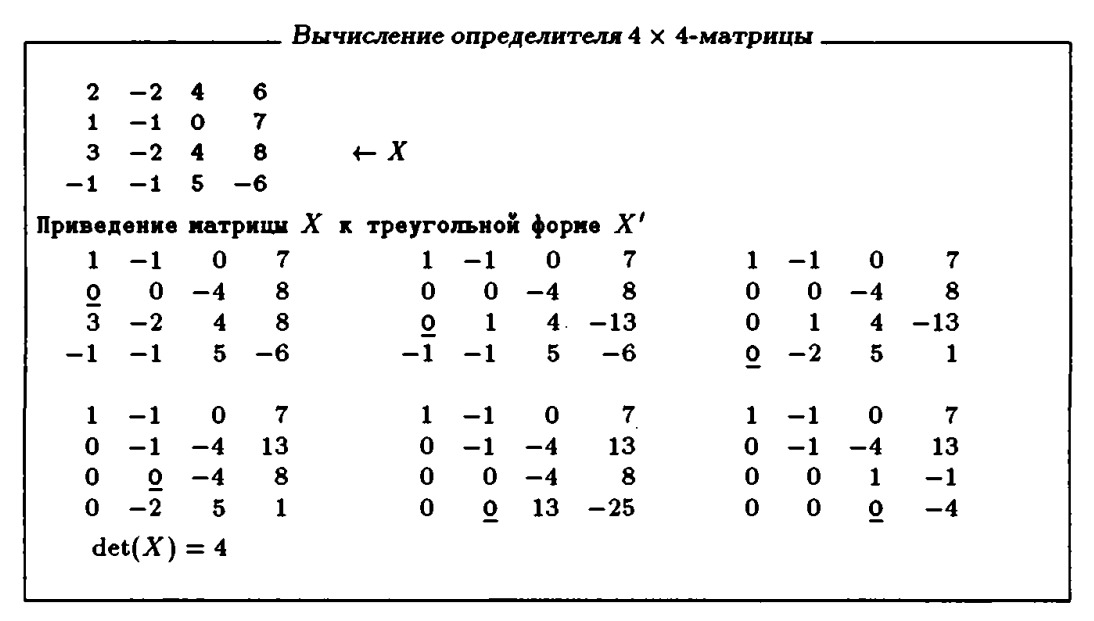
\includegraphics[width=1\linewidth]{image2}}
\end{figure}

Этот метод позволяет получить результаты с более разумным вре- \linebreak менем вычисления: на микрокалькуляторе типа AT время вычисления \linebreak определителя матрицы размеров $10 \times 10$ порядка 20 секунд (для на- \linebreak ивного метода было нужно более часа вычислений). Наконец, чтобы \linebreak убедиться в справедливости вычислений (никто не застрахован от оши-\linebreak
%317
\noindent бок), мы вычислили снова определители Майе!:  
$$h*(p)=h_1(p)=|\det (X_{ij})_{3 \le i, j \le (p-1)/2}|, X_{ij}=\lfloor{\frac{ij}{p}}\rfloor - \lfloor{\frac{(i-1)j}{p}}\rfloor,$$
для простого $p \le 47$ и сравнили полученные нами значения со значени- \linebreak ями, встречающимися в литературе. Эти определители имеют большое \linebreak значение в теории чисел. В действительности, существует целое поло- \linebreak жительное число, обозначаемое $h(p)$, которое измеряет степень неглав- \linebreak ности кольца $\mathbb{Z}[\sqrt[p]{1}]$ целых циклотомических чисел: $h(p)$ — число клас- \linebreak сов идеалов кольца $\mathbb{Z}[\sqrt[p]{1}]$. Сказать, что это кольцо — КГИ, равнозначно \linebreak тому, что $h(p) = 1$. Разумеется, можно разложить $h(p)$ в произведение \linebreak $h(p) = h_1(p)h_2(p)$ где $h_1(p)$ и $h_2(p)$ названы, соответственно, первым \linebreak и вторым множителем числа классов $\mathbb{Z}\sqrt[p]{1}$. Число $h_1(p)$, обозначаемое \linebreak также $h^*(p)$ и $h^-(p)$ (число $h_2(p)$ обозначается также $h^+(p)$), обладает \linebreak следующим фундаментальным свойством:
$$p \nmid h^*(p)\Longleftrightarrow p \nmid h(p),$$
$$p \nmid h^*(p) \Rightarrow \text{великая} \ll \text{ теорема } \gg \text{Ферма истинна для показателя } p,$$
указанная теорема утверждает, что уравнение $x^p + y^p = z^p$ не имеет \linebreak целых строго положительных решений для простых $p \ge 3$.
  
Интересующийся этим вопросом читатель может обратится к ра- \linebreak боте Рибенбойма $[153]$, в которой фигурирует таблица чисел $h^*(p)$ для \linebreak простых $p \le 163$, вычисленная вручную Куммером во второй поло- \linebreak вине 19-ого века. Здесь найдено простое число $p$, для которого $\mathbb{Z}[\sqrt[p]{1}]$ не \linebreak будет КГИ ($р = 23$), и простое нерегулярное число $p$, т.е. такое, что $p$ \linebreak делит $h^*(p)$ ($p = 37$). Эта таблица дает, в то же время, порядок размера \linebreak чисел $h^*(p)$: например, $h^*(149) = 3^2 \times 149 \times 512966338320040805461$.
\subsection{Модули без кручения конечного типа.}
\noindent Вот другое более абстрактное применение леммы исключения.

\begin{predl}
Пусть $M$ — $A$-модуль \textbf{конечного типа}, т.е. порожденный конеч- \linebreak ным числом образующих, и \textbf{без кручения)}(т.е. для $a \in A$, $x \in X$,\linebreak $ax=0 \Rightarrow a=0$ или $x=0$) над \textbf{КГИ} $A$. Обозначим через $\rho(M)$ мини- \linebreak мальное число элементов в системе образующих $M$. Тогда  
(i) любая порождающая $M$ система элементов, имеющая $\rho(M)$ эле- \linebreak ментов, свободна,  
(ii) в частности, $М$ свободен.  \newpage
%318
Отметим, что минимальная система образующих необязательно яв- \linebreak ляется системой с минимальным числом элементов. Рассмотрите, на- \linebreak пример, минимальную систему образующих $(2,3)$ в $\mathbb{Z}$.
\end{predl} 
\begin{lemma}
Пусть $A$ --- кольцо главных идеалов, $x_1, x_2, ..., x_n$ --- $n$ элементов \linebreak $A$ --- модуля $M$, $a_1, a_2, ..., a_n$ --- $n$ элементов кольца $А$. Тогда существуют \linebreak $x_1', х_2', ..., x_n'$ в $M$, удовлетворяющие условию:  
$$Ax_1 + Ax_2 + ... + Ax_n = Ax_1' + Ax_2' + ... + Ax_n' и a_1x_1 + a_2x_2 + ... + a_nx_n = dx_1',$$
$d \in A$ обозначает НОД элементов $a_1, a_2, ..., a_n$.
\end{lemma}
\begin{myproof}
В силу индукции достаточно рассмотреть лемму для $n=2$; по лем- \linebreak ме исключения существует матрица ${\left( \begin{array}{ccc}
\alpha & \beta \\
\gamma & \delta \\
\end{array} \right)} \in SL(2,A)$, удовлетворя- \linebreak ющая условию:  
$${\left( \begin{array}{ccc}
d & 0 \\
\end{array} \right)}{\left( \begin{array}{ccc}
\alpha & \beta \\
\gamma & \delta \\
\end{array} \right)}={\left( \begin{array}{ccc}
a_1 & a_2 \\
\end{array} \right)},$$
$d$ — НОД$(a_1, a_2)$. Достаточно определить $x_1', x_2' \in M$:
$${\left( \begin{array}{ccc}
x_1' \\
x_2' \\
\end{array} \right)}={\left( \begin{array}{ccc}
\alpha & \beta \\
\gamma & \delta \\
\end{array} \right)}{\left( \begin{array}{ccc}
x_1 \\
x_2 \\
\end{array} \right)}.$$
Это равенство можно преобразовать (матрица обратима), доказав, \linebreak что $Ax_1+ Ax_2= Ax_1' + Ax_2'$ . Тогда имеют место равенства:  
$$a_1x_1 + a_2x_2 = {\left( \begin{array}{ccc}
a_1 & a_2 \\
\end{array} \right)}{\left( \begin{array}{ccc}
x_1 \\
x_2 \\
\end{array} \right)} = {\left( \begin{array}{ccc}
a_1 a_2 \\
\end{array} \right)} {\left( \begin{array}{ccc}
\alpha & \beta \\
\gamma & \delta \\
\end{array} \right)}^{-1}{\left( \begin{array}{ccc}
x_1' \\
x_2 '\\
\end{array} \right)} = {\left( \begin{array}{ccc}
d & 0\\
\end{array} \right)} {\left( \begin{array}{ccc}
x_1' \\
x_2'\\
\end{array} \right)} = dx_1',$$
что и требовалось доказать.
\end{myproof}
\noindent\textbf{Доказательство предложения 9}


Пусть $\{x_1, x_2,..., x_n\}$ порождающее подмножество модуля $M$, со- \linebreak стоящее из $n = \rho (M)$ элементов. Рассмотрим соотношение зависимо- \linebreak сти $a_1x_1 + a_2x_2 + ... +a_nx_n = 0$. Докажем, что все $a_i$ нулевые, и, как \linebreak следствие, что $\{x_1, x_2, ..., x_n\}$ --- базис $М$.  \newpage
%319
В силу предыдущей леммы существует семейство образующих \linebreak $\{x_1', x_2',..., x_n'\}$ в $M$ такое, что $dx_1' = 0$, $d$ --- наибольший общий дели- \linebreak тель $a_1, a_2, ..., a_n$. Здесь $x_1'$ \textbf{не нуль}, иначе семейство $x_2', x_3', ..., x_n'\}$ \linebreak было бы семейством образующих, имеющим строго меньше, чем $\rho (M)$ \linebreak элементов. То, что $M$ без кручения, влечет, что $d$ --- нуль, и, как след- \linebreak ствие, что все $a_i$ нулевые. Это доказывает (i)  и (ii).

\section{Нормальная форма подгруппы группы $\mathbb{Z^n}$}
\noindent Сейчас мы продемонстрируем более общие результаты,чем сформули- \linebreak рованные (для $\mathbb{Z^2}$) во введении к этой главе и касающиеся представле- \linebreak ния в каноническом виде подгрупп $\mathbb{Z^n}$.

\subsection{Исследование подгруппы $n\mathbb{Z} \times m\mathbb{Z}$ группы $\mathbb{Z^2}$}
\noindent Целью наших действий в этом частном случае является стремление \linebreak объяснить читателю некоторые составные части теории инвариантных \linebreak множителей. Во введении мы установили существование изоморфизма \linebreak между абелевыми группами $\mathbb{Z_n} \times \mathbb{Z_m}$ и $\mathbb{Z_{n \wedge m}} \times \mathbb{Z_{n \vee m}}$; оно базировалось \linebreak на разложении чисел $n$ и $m$ в произведение простых множителей, и в \linebreak явном виде представлено на было; сделаем это сейчас.
  
Основная идея состоит в том, чтобы сконцентрироваться на поло- \linebreak жении подгруппы $n\mathbb{Z} \times m\mathbb{Z}$ в $\mathbb{Z} \times \mathbb{Z}$, забыв ненадолго про произведение \linebreak $\mathbb{Z_n} \times \mathbb{Z_m}$. Важно убедиться, что группа $n\mathbb{Z} \times m\mathbb{Z}$ изучена в окружающем \linebreak пространстве $\mathbb{Z}\times \mathbb{Z}$. Чтобы понять этот основной нюанс, рассмотрим \linebreak две подгруппы $2\mathbb{Z} \times \mathbb{Z}$ и $3\mathbb{Z} \times \mathbb{Z}$ группы $\mathbb{Z}^2$. Эти две подгруппы, очевид- \linebreak но, изоморфны, но между тем, не существует изоморфизма $\mathbb{Z}^2$ на себя,\linebreak переводящего первую группу во вторую (почему?).
  
Следующий результат, применимый к произведению двух цикличе- \linebreak ских групп, является более общим и более конструктивным, чем резуль- \linebreak тат, приведенный во введении.  
\begin{predl}
Пусть $n$ и $m$ два целых числа, $d = n \wedge m$, $p = n \vee m$. Существует \linebreak квадратная матрица $L$ порядка 2 с целыми коэффициентами и с опре- \linebreak делителем 1, представляющая автоморфизм $\mathbb{Z} \times \mathbb{Z}$ и удовлетворяющая \linebreak следующему условию: $L(n\mathbb{Z} \times m\mathbb{Z}) = d\mathbb{Z} \times p\mathbb{Z}$. Кроме того, эта матрица \linebreak легко выражается в явном виде.
\end{predl}
\newpage
%320
\begin{myproof}
Отметим еще раз, что построение такой матрицы основано на со- \linebreak отношении Безу. Можно предположить, что одно из двух целых \linebreak чисел $n$ или $m$ не нулевое; пусть $d = un +vm$ --- отношение Безу \linebreak и положим $\tilde{n} = n/d$ и $\tilde{m} = m/d$ при условии, что $u\tilde{n} + v\tilde{m} = 1$,\linebreak $\tilde{n}m = \tilde{m}n = p$. Матрица $L = {\left( \begin{array}{ccc}
u & v \\
-\tilde{m} & \tilde{n} \\
\end{array} \right)}$ , которая уже фигури- \linebreak ровала в лемме исключения, — искомая: ее определитель, конечно, \linebreak равен 1, и можно легко показать, что $(d, 0)$ и $(0, p)$ принадлежат \linebreak $L(n\mathbb{Z} \times m\mathbb{Z})$, т.е. что $d\mathbb{Z} \times p\mathbb{Z} \subset L(n\mathbb{Z} \times m\mathbb{Z})$. Можно также по- \linebreak казать, что $L(n\mathbb{Z} \times m\mathbb{Z})\subset d\mathbb{Z} \times p\mathbb{Z}$. Это доказывает равенство в \linebreak формулировке предложения.
\end{myproof}
\begin{sled}
В соответствии с предыдущими обозначениями, матриц \linebreak $L = {\left( \begin{array}{ccc}
u & v \\
-\tilde{m} & \tilde{n} \\
\end{array} \right)}$ и обратная матрица $L^{-1} = {\left( \begin{array}{ccc}
\tilde{n} & -v \\
\tilde{m} & u \\
\end{array} \right)}$ индуцируют \linebreak изоморфизмы $\overline{L}$ из $\mathbb{Z}_n \times \mathbb{Z}_m$ в $\mathbb{Z}_d \times \mathbb{Z}_p$ и $\overline{L^{-1}}$ из $\mathbb{Z}_d \times\mathbb{Z}_p$ в $\mathbb{Z}_n \times \mathbb{Z}_m$ \linebreak (каждая, соответственно). 
Можно еще улучшить предыдущие результаты:  
$${\left( \begin{array}{ccc}
d & 0 \\
0 & p \\
\end{array} \right)} = L {\left( \begin{array}{ccc}
n & -vp \\
m & up \\
\end{array} \right)} = L {\left( \begin{array}{ccc}
n & 0 \\
0 & m \\
\end{array} \right)}{\left( \begin{array}{ccc}
1 & -v\tilde{m} \\
1 & u\tilde{n} \\
\end{array} \right)} = {\left( \begin{array}{ccc}
n & 0 \\
0 & m \\
\end{array} \right)}R,$$
где  $R = {\left( \begin{array}{ccc}
1 & -v\tilde{m} \\
1 & u\tilde{n} \\
\end{array} \right)}$ --- $2 \times 2$ - матрица с целыми коэффициентами и с \linebreak определителем 1. Как следствие имеем: 
\end{sled}
\begin{predl}
Используя предыдущие обозначения, можно выразить в явном виде \linebreak $2 \times 2$ - матрицы $R$ и $L$ с определителями 1, удовлетворяющие условию: 
${\left( \begin{array}{ccc}
d & 0 \\
0 & p \\
\end{array} \right)} =  L{\left( \begin{array}{ccc}
n & 0 \\
0 & m \\
\end{array} \right)}R, где d делит p.$
\end{predl}
\begin{mynotice}
Раньше считали этот результат более сильным, чем \linebreak предыдущие. В действительности же, интерпретируя $n \mathbb{Z} \times m \mathbb{Z}$ \linebreak как образ диагональной матрицы ${\left( \begin{array}{ccc}
n & 0 \\
0 & m \\
\end{array} \right)}$ получаем, что равенство \linebreak матриц, объявленное в предложении 13, влечет равенство   
$$L(n\mathbb{Z} \times m\mathbb{Z}) = d\mathbb{Z} \times p\mathbb{Z}$$
\end{mynotice}
\newpage
%321
Действительно, этот последний результат является частным случа- \linebreak ем следующей более общей теоремы, которая будет доказана позже и \linebreak которая ведет к классификации абелевых групп конечного типа.  
\begin{thm}
Пусть дана квадратная $q \times q$-матрица $А$ с целыми элементами. Мож- \linebreak но предъявить две $q \times q$-матрицы $L$ и $R$ с целыми элементами и с опре- \linebreak делителем 1 такие, что $B = LAR$ будет диагональной матрицей и вы- \linebreak полняется условие:  
$$b_{11}|b_{22}, b_{22}|b_{33}, ..., b_{q-1 q-1}|b_{qq},$$
и, как следствие, переходя к частному, $\mathbb{Z}^q / ImA \simeq \mathbb{Z}_{b_{11}} \times \mathbb{Z}_{b_{22}} \times ... \times \mathbb{Z}_{b_{qq}}.$
\end{thm}
\subsection{Изучение подгруппы $a_1\mathbb{Z} \times ... \times a_n\mathbb{Z}$ группы $\mathbb{Z^n}$}
\noindent Этот параграф, посвященный изучению конечного произведения \linebreak $\mathbb{Z_{a_1}} \times \mathbb{Z_{a_2}} \times ... \times \mathbb{Z_{a_n}}$ циклических групп, должен позволить читате- \linebreak лю близко познакомиться с понятием инвариантных множителей: как \linebreak и в случае $n = 2$ в предыдущем разделе, мы будем изучать положение подгруппы $\mathbb{Z_{a_1}} \times \mathbb{Z_{a_2}} \times ... \times \mathbb{Z_{a_n}}$ в группе $\mathbb{Z^n}$.

\begin{determ}
\
 \begin{description} \item[(i)]  Две последовательности целых чисел $(a_1, a_2, ..., a_n)$ и \linebreak $(b_1, b_2, ..., b_m)$ называются \textbf{эквивалентными}, если существует изо- \linebreak морфизм $\varphi : \mathbb{Z^n} \to \mathbb{Z^m}$, переводящий подгруппу $\mathbb{Z_{a_1}} \times \mathbb{Z_{a_2}} \times ... \times \mathbb{Z_{a_n}}$ в \linebreak подгруппу $\mathbb{Z_{b_1}} \times \mathbb{Z_{b_2}} \times ... \times \mathbb{Z_{b_m}}$ (это незамедлительно влечет равенство \linebreak $n = m$, как мы увидим в следствии 19).  
\item[(ii)] Последовательность целых чисел $a_1, a_2, ..., a_n$ называется \textbf{нор-} \linebreak \textbf{мализованной}, если $a_1 | a_2 | a_3 | ... | a_{n-1} | a_n$.   
Если две последовательности целых чисел $(a_1, a_2, ..., a_n)$ и \linebreak $(b_1, b_2, ..., b_m)$ эквивалентны, то $n = m$ и --- что больше всего нас инте-\linebreak ресует, --- факторгруппы $\mathbb{Z_{a_1}} \times \mathbb{Z_{a_2}} \times ... \times \mathbb{Z_{a_n}}$ и $\mathbb{Z_{b_1}} \times \mathbb{Z_{b_2}} \times ... \times \mathbb{Z_{b_m}}$ изо- \linebreak морфны. Достаточно перейти к частным для изоморфизма из пункта \linebreak \item[(i)] . Заметим, что при переходе к частным, каждое $a_i$, равное 1 или -1, \linebreak соответствует тривиальному фактору $\mathbb{Z} / \mathbb{Z}$, который можно опустить.

\end{description} 
\end{determ}
\emph{\textbf{(16) Предложение.}}

Существует алгоритм, который, будучи применен к последователь- \linebreak ности целых чисел $a_1, a_2, ..., a_n$, строит \textbf{нормализованную} последо- \linebreak вательность $b_1, b_2, ..., b_n$, \textbf{эквивалентную} исходной.  \newpage
%322
В частности, для конечного произведения $\mathbb{Z_{a_1}} \times \mathbb{Z_{a_2}} \times ... \times \mathbb{Z_{a_n}}$ ци- \linebreak клических групп изоморфизм с произведением $\mathbb{Z_{b_1}} \times \mathbb{Z_{b_2}} \times ... \times \mathbb{Z_{b_m}}$, где \linebreak $b_i$ --- целые числа, отличные от 1 и -1, и $b_i$ делят $b_{i+1}$, может быть \linebreak выражен в явном виде.

\begin{lstlisting}[mathescape=true]

  $b \in \mathbb{Z}^n$ Normaliser $(a \in \mathbb{Z}^n)$
  $b = (b_1, b_2, ..., b_n) \gets (a_1, a_2, ..., a_n)=a;$
  for($i = 1$; $i < n-1$; $++i$)
      for ($j=i+1$; $j<n$; $++j$)
          $(b_i, b_j) \gets (b_i ) \wedge b_j, b_i \vee b_j);$
      

  return $(b_1, b_2, ..., b_n);$

\end{lstlisting}
\begin{myproof}\linebreak
Это доказательство основано на программной обработке, можно \linebreak также обратиться к упражнению 18. Уточним сейчас, что исполь- \linebreak зуемый метод не основан на разложении целых чисел $a_i$ в произве- \linebreak дение простых сомножителей: единственное, что используется, --- \linebreak это наибольший общий делитель $\wedge$ и наименьшее общее кратное $\vee$.\linebreak Пусть даны два индекса $i < j$; из результатов предыдущего раздела \linebreak понятно, что:  
$$(a_1,...,a_i,...,a_j,...,a_n) \sim (a_1,...,a_i \wedge a_j,...,a_i \vee a_j,...,a_n),$$
$\sim$ символизирует эквивалентность последовательностей, фигуриру-\linebreak ющих в определении 15.  

\noindent Назовем $E_{ij}$ операцию, которая состоит в замене первой из этих \linebreak последовательностей на вторую. Тогда ясно, что, если выполнить \linebreak последовательно операции $E_{12}, E_{13}, E_{14}, ..., E_{1n}$, то получится по- \linebreak следовательность $a'$, эквивалентная исходной и удовлетворяющая,\linebreak кроме того, условиям делимости $a_1'|a_2', a_1'|a_3', ..., a_1'|a_n'$ (дей- \linebreak ствительно, $a_1'$ --- НОД элементов исходной последовательности).\linebreak Затем можно применить к подпоследовательности $(a_2', a_3',..., a_n')$\linebreak операции $E_{23}, E_{24}, ..., E_{2n}$, после чего получим, очевидно, \linebreak эквивалентную подпоследовательность, удовлетворяющую условию \linebreak $a_2''|a_3'', a_2''|a_4'', ..., a_2''|a_n''$ и, к тому же, $a_1'|a_2''$ (потому что $a_2''$ \linebreak является НОД $a_i'$, каждое из которых делится на $a_1'$).  \newpage
%323

\noindent Применяя $n-1$ раз этот процесс (последней операцией будет \linebreak $E_{n, n-1}$), получаем последовательность, эквивалентную начальной и \linebreak нормализованную. Алгоритм 2 нормализации вытекает из этих рас- \linebreak суждений.
\end{myproof}
Интерпретация на языке Ада, которая приводится ниже, основа- \linebreak на не на функции, как в алгоритме, описанном выше, а на процедуре. \linebreak Эта процедура имеет только один параметр типа in out. Цель это-\linebreak го алгоритма, кроме нормализации последовательностей целых чисел, \linebreak построить след всего процесса нормализации.
\begin{lstlisting}[mathescape=true]
 #include<stdio.h>
 #include<stdlib.h>
 int n;   
 void Trace_Normalization (b : Module_Representation) {
    for(i=$b'First$; $i<b'Last-1$; ++i){
        for($j=i+1$; $j<b'Last$; ++j){
            b(i):=GCD_bi_bj;
            if (GCD_bi_bj = 0) 
            {
                b(j):=0; 
            } 
            else 
            {    
                b(j):=(bi/GCD_bi_bj)^*bj;

        
  void Get (a: Module_Representation){
      for(k=0; k<a; ++k){
          scanf("%d",&(a(k)));
      }
      while( true) {
          printf("Длина представления : ");
          scanf("d", &n);
          a= Module_Representation (1 .. n);
          printf("представление : ");
          scanf("%d", &a);
          printf("Данное представление : ");
          printf("%d", a);
          printf("%d", b);
          printf("Приведение : ");
          Trance_Normalization (a);
          if (Data_Error => NULL){
              break;          
\end{lstlisting}
\newpage
Вот только несколько примеров применения предыдущей прог- \linebreak раммы. 
\begin{figure}[h]
\center{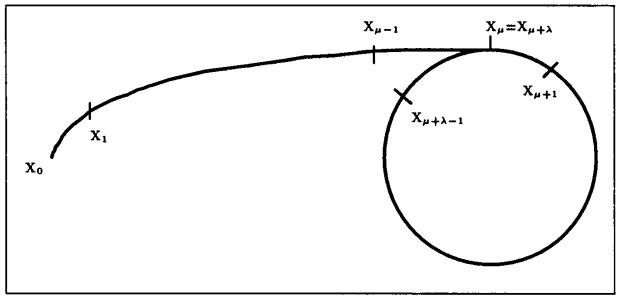
\includegraphics[width=1\linewidth]{image3}}
\end{figure}
\noindent А теперь выделим все основные понятия теории инвариантных множителей: матрицы с целыми коэффициентами, подгруппы образов,\linebreak факторгруппы $\mathbb{Z}^g/ImA$, нормализованные формы...  
\subsection{Единственность нормального разложения}
\noindent В предыдущем разделе мы показали, что любое произведение $\mathbb{Z}_n \times \mathbb{Z}_m$ \linebreak можно всегда заменить, используя изоморфизм, другим произведением \linebreak $\mathbb{Z}_{n'} \times \mathbb{Z}_{m'}$, где $n'$ делит $m'$. Но среди всех способов записи $\mathbb{Z}_n \times \mathbb{Z}_m$ в \linebreak виде произведения двух циклических групп лучший, когда $n$ делит $m$. 
\\
\\
\textbf{Пример}
\\

Рассмотрим группу, имеющую 48 элементов, представленную в виде \linebreak произведения двух циклических групп, $\Omega = \mathbb{Z}_{2} \times \mathbb{Z}_{24}$ . Числа 24 и 2 можно \linebreak найти, \textbf{зная только структуру группы $\Omega$}. Действительно, число 24 \linebreak получено следующим образом:   
 $$24\mathbb{Z} = \{ q \in \mathbb{Z} \text{ удовлетворяющие условию } qx = 0 , \forall x \in \Omega\} =$$ $$
= \{g \in \mathbb{Z},\text{ удовлетворяющие условию } q\Omega = \{0\}\}.$$

Это можно записать (выражение в фигурных скобках является опреде- \linebreak лением слова аннулятор): $24\mathbb{Z}$ = аннулятор($\Omega$). Что касается числа 2, \linebreak оно находится из равенства $2 \times 24$ = порядок($\Omega$). Таким образом, абеле- \linebreak ва группа ${\Omega}' = \mathbb{Z}_4 \times \mathbb{Z}_{12}$ имеет порядок в точности 48, но ее аннулятор --- \linebreak $12\mathbb{Z}$, поэтому ${\Omega}'$ не может быть изоморфна группе $\Omega = \mathbb{Z}_2 \times \mathbb{Z}_{24}$ (две \linebreak изоморфные группы имеют равные аннуляторы). 
\begin{predl}

Пусть $n, m, n'$ и $m'$ --- четыре элемента из $\mathbb{Z}$ такие, что $n | m$,\linebreak $n' | m'$ и $\mathbb{Z}_n \times \mathbb{Z}_m \simeq \mathbb{Z}_{n'} \times \mathbb{Z}_{m'}$. Тогда $n = \pm n'$, $m = \pm m'$; это можно \linebreak также записать в виде $n\mathbb{Z} = n'\mathbb{Z}$ и $m\mathbb{Z} = m' \mathbb{Z}$. 

На этой стадии, вдохновленный предыдущим примером\linebreak ($\Omega = \mathbb{Z}_2 \times \mathbb{Z}_{24}$, читатель может доказать теорему единственности, по \linebreak крайней мере в случае, когда $n, m, n', m'$ не нули. Заметим однако, что \linebreak этот результат единственности говорит также, что $\mathbb{Z} \times \mathbb{Z}$ не изоморфна \linebreak $\mathbb{Z}$, но это уже другая история. 

Сейчас мы докажем теорему единственности, имеющую очень широ- \linebreak кий спектр действия. Технические методы отличны от методов, исполь- \linebreak зуемых в частном случае в предыдущем примере: вместо аннуляторов \linebreak мы будем использовать минимальное число образующих для модулей \linebreak конечного типа.
%326
\end{predl}
\begin{thm}[единственности.]

$A$ обозначает \textbf{коммутативное} унитарное кольцо. Пусть \linebreak $I_1, I_2, ..., I_p$ и $J_1, J_2, ..., J_p$ --- \textbf{собственные} идеалы кольца $A$, удо- \linebreak влетворяющие условию: 
$$I_p \subset I_{p-1}\subset ... \subset I_1, J_p \subset J_{q-1}\subset ... \subset J_1$$
$$и A/I_1 \times A/I_2 \times ... \times A/I_p \simeq A/J_1 \times A/J_2 \times ... \times A/J_p$$
Тогда $p = q$ и $I_i = J_i$ для $i = 1, 2, ...$ 
\end{thm}
\begin{sled}
Пусть A — коммутативное унитарное кольцо; если $p$ и $q$ таковы, \linebreak что $A^p$ изоморфно $A^q$, тогда $p = q$ (непосредственное применение пре- \linebreak дыдущей теоремы в случае, когда идеалы нулевые). 

Чтобы доказать теорему 18, необходимо использовать несколько \linebreak лемм. Но прежде всего несколько комментариев о предпосылках тео- \linebreak ремы.
\end{sled}
\begin{mynotice} То, что все идеалы будут предполагаться отличны- \linebreak ми от А, позволяет избежать появления тривиальных множителей \linebreak $A/A$; кроме того, условие на цепи идеалов является необходимым, \linebreak как это показывает пример $\mathbb{Z}_2 \times \mathbb{Z}_3 \simeq \mathbb{Z}_6$. 

Если идеалы главные, $I_1 = (a_1), I_2 = (a_2), ...,$\linebreak $I_p = (a_p)$, то условие на цепи эквивалентно отношениям дели- \linebreak мости:
$$a_1 | a_2 | a_3 ... a_{p-1} | a_p.$$ 

Основное кольцо предполагается коммутативным и фунда- \linebreak ментальным. В действительности существуют не коммутативные \linebreak унитарные кольца А, такие, что $A \simeq A^2$ как A-модули. Рассмо- \linebreak трим, например, векторное $\mathbb{Q}$-пространство конечных последова- \linebreak тельностей из $\mathbb{N}$ в $\mathbb{Q}$ и кольцо А эндоморфизмов из $\mathbb{Q}^{\mathbb{N}}$. Пусть $u$ \linebreak и $v$ — два элемента из A, определенные их действием на канони-\linebreak ческом базисе: 
$$u(e_{2n}) = e_n, u(e_{2n+1}) = 0, v(e_{2n}) = 0, v(e_{2n+1}) = e_n.$$
Тогда имеем: $A = Au \oplus Av$. Чтобы это доказать, достаточно рас- \linebreak смотреть отображения $U$ и $V$, отвечающие $u$ и $v$ соответственно, \linebreak такие, что $U(e_n) = e_{2n}$, $V(e_n) = e_{2n + 1}$, значит $uU = vV = Id$.\linebreak Нетрудно видеть, что в этом случае $Id = Uu + Vv$.
\end{mynotice}
\begin{lemma}
Пусть дан A-модуль М конечного типа, обозначим через $\rho(M)$ наи- \linebreak меньшее число образующих из М.  
%327
Пусть $I_1 \supset I_2 \supset ... \supset I_p$ --- цепь собственных идеалов в А. Тогда \linebreak $\rho(A/I_1 \times A/I_2 \times ... \times A/I_p) = p.$
\end{lemma}
\begin{myproof}
Теорема Крулля утверждает существование максимального идеала \linebreak $\mathcal{M}$, содержащего собственный идеал $I_1$
 (если $A = \mathbb{Z}$ и $I_1 = (a_1)$, то \linebreak этот идеал --- $(q)$, где $q$ — простой делитель $a_1$). Этот идеал будет \linebreak самым большим в цепи. Применим тогда сюръективное отображе- \linebreak ние:

$$\pi:A/I_1 \times A/I_2 \times ... \times A/I_p \to {(A/ \mathcal{M})}^p,$$
которое является произведением канонических отображений \linebreak $A/I_i \to A/ \mathcal{M}$. Если $S$ --- система образующих в $A/I_1 \times A/I_2 \times$ \linebreak $... \times A/I_p$, то $\pi(S)$ --- система образующих векторного $A/\mathcal{M}$- \linebreak пространства ${(A/\mathcal{M})}^p$ и, следовательно, $card \; S \; \ge \; card \; \pi(S) \; \ge$ \linebreak $dim{(A/ \mathcal{M})}^p = p$. Любая система образующих в $A/I_1 \times A_/I_2 \times ... \times$ \linebreak $A/I_p$ содержит по крайней мере $p$ элементов. К тому же, семейство \linebreak $e_1 = (\overline{1}, 0, ..., 0), e_2 = (0, \overline{1}, 0, ..., 0), ..., e_p = (0, ..., 0, \overline{1})$ --- система \linebreak образующих в $A/I_1 \times A/I_2 \times ... \times A/I_p$, имеющая ровно $p$ элементов.\linebreak Следовательно,  
$$\rho(A/I_1 \times A/I_2 \times ... \times A/I_p) = p.$$
\end{myproof}
\begin{lemma}
Пусть $I$ — идеал в $A$ и $b \in A$. Существует канонический изоморфизм \linebreak $bA/I \simeq A/I^b$, идеал $I^b$ определяется как $I^b = \{x \in A | bx \in I\}.$ 
\end{lemma}
\begin{myproof}
Отображение $A \to bA/I$, которое элементу $x \in A$ ставит в соот- \linebreak ветствие элемент $b\overline{x} \in bA/I$ является сюръективным с ядром $I^b$ и \linebreak индуцирует изоморфизм между A-модулями $bA/I$ и $A/I^b$.\par
\end{myproof}
\textbf{Доказательство теоремы 18}

Пусть $P = A/I_1 \times A/I_2 \times ... \times a/I_p$ и $Q = A/J_1 \times A/J_2 \times ... \times A/J_q$. \linebreak В силу леммы 20, $p = \rho(P)$.\par

Докажем равенство $I_1 = \{b \in A | \rho(bP) \le p - 1\}$. По предыдущей \linebreak лемме имеет место равенство:\par
$$bP \simeq A/{I_1}^b \times A/{I_2}^b \times ... \times A/{I_p}^b, \text{где } {I_1}^b \supset {I_2}^b \subset ... \subset {I_p}^b.$$
\newpage
